%!TEX program = xelatex
\documentclass[cn,hazy,blue,14pt,normal]{elegantnote}
\title{电磁学}

\author{Jaden Feng\\冯杰骏}

\date{}

\usepackage{CJKfntef}
\usepackage{array}
\usepackage{physics}
\usepackage{esint}
\usepackage{amsmath}
\numberwithin{equation}{section}
\usepackage{amssymb}
\usepackage{wrapfig}
\usepackage{tikz}
\usetikzlibrary{arrows, positioning, calc, angles, quotes}

\begin{document}

\maketitle
\pagenumbering{roman}
\setcounter{page}{1}
\newpage
\begin{center}
    \Huge\textbf{{Introduction}}\\
\end{center}~\
电磁学笔记。
\begin{flushright}
    \begin{tabular}{c}
        Jaden Feng\\
        冯杰骏\\
        \date{\today}
    \end{tabular}
\end{flushright}

\newpage
\pagenumbering{Roman}
\setcounter{page}{1}
\tableofcontents

\newpage
\setcounter{page}{1}
\pagenumbering{arabic}

\section{静电场的基本规律}
\newpage
\subsection{库仑定律}
\begin{theorem}
  库仑定律:
\end{theorem}
\begin{equation}
  \vec{F}=\frac{1}{4\pi\varepsilon_0}\frac{q_1q_2}{r^2}\vec{e_r}
\end{equation}
因为 $\vec{E}\equiv\frac{\vec{F}}{q}$ :
\begin{equation}\label{点电荷电场}
  \begin{aligned}
    \vec{E}&=\frac{1}{4\pi\varepsilon_0}\frac{Q}{r^2}\vec{e_r}\\
    &=\frac{1}{4\pi\varepsilon_0}\iiint\frac{\rho\ \dd V}{r^2}\vec{e_r}
  \end{aligned}
\end{equation}
$Q$ 是场源电荷电荷量,$\rho$ 是电荷体密度, $\vec{e_r}$ 方向是源点 $\to $ 场点。\\
\begin{example}\label{example1.1}
  例题:求无限长带电直线中垂面上的电场分布。
\end{example}

\begin{wrapfigure}{r}{0.2\textwidth}
  \begin{tikzpicture}
    % 绘制无限长直线
    \draw(0,-2) -- (0,2) node[above] {$\infty$};
    \draw(0,2) -- (0,-2) node[below] {$\infty$};
  
    % 标记点 Q 和 q
    \fill (0,0) circle (2pt) node[left] {$Q$};
    \fill (2,0) circle (2pt) node[below right] {$q$};
  
    % 连接 Q 和 q,并标记距离 r
    \draw[dashed] (0,0) -- (2,0) node [midway,above]{$r$};
  \end{tikzpicture}
\end{wrapfigure}
\noindent
Establish the y-axis along the direction of the line, and establish the x-axis perpendicular to the direction of the line.
\\
$$
\text{d}\vec{E}=\frac{1}{4\pi\varepsilon_0}\frac{\lambda\dd l}{r^2}\vec{e_r}
$$
\\
According to symmetry, the components of the upper and lower part on the y-axis cancel each other out. \\
If the y-component is required, simply replace $\cos\alpha$ with $\sin\alpha$ in the following equation.
\\
$$
\dd E_x=\frac{1}{4\pi\varepsilon_0}\frac{\lambda\dd l}{r^2}\cos \alpha
=\frac{1}{4\pi\varepsilon_0}\frac{\lambda R\dd l}{(R^2+l^2)^{\frac{3}{2}}}
$$
\\
Integral:
\begin{align*}
	E_x&=\int^{+\infty}_{-\infty}\frac{1}{4\pi\varepsilon_0}\frac{\lambda R}{(R^2+l^2)^{\frac{3}{2}}}\dd l\\
	&=\frac{\lambda R}{4\pi\varepsilon_0}\int^{+\infty}_{-\infty}\frac{1}{(R^2+l^2)^{\frac{3}{2}}}\dd l
\end{align*}

\begin{wrapfigure}{r}{0.3\textwidth}
  \begin{center}
  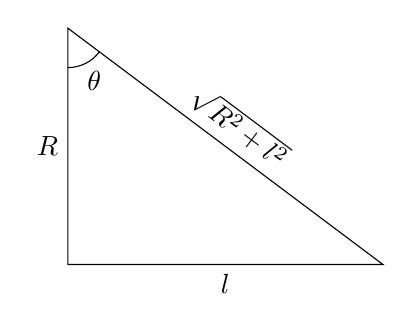
\begin{tikzpicture}
    % Put R and l into a right triangle, and let them be the adjacent side
    \def\R{3}
    \def\l{4}
    % 绘制三角形
    \coordinate (A) at (0,0);
    \coordinate (B) at (0,\R);
    \coordinate (C) at (\l,0);
    \draw (A) -- (B) node[midway, left] {$R$} -- (C)  -- cycle node[midway, below] {$l$};
    % 标记斜边长度
    \path (B) -- (C) node[midway, above, sloped] {$\sqrt{R^2 + l^2}$};
    % 标记角度 theta
    \pic [draw, "$\theta$", angle eccentricity=1.5] {angle = A--B--C};
  \end{tikzpicture}
  \end{center}
\end{wrapfigure}
\noindent
We define the angle between the adjacent side whose length is R and the hypotenuse as $\theta$​
\\
Then we get:
\begin{equation*}
  \begin{split}
    \cos\theta = \frac{R}{\sqrt{R^2+l^2}}\quad &\Longrightarrow\quad\frac{\cos^3\theta}{R^3}
=\frac{1}{(R^2+l^2)^{\frac{3}{2}}}\\
l=R\tan\theta\quad &\Longrightarrow\quad\dd l=\frac{R}{\cos^2\theta}\dd\theta
  \end{split}
\end{equation*}
\\
Then:
\begin{align*}
	E_x&=\frac{\lambda R}{4\pi\varepsilon_0}\int^{+\infty}_{-\infty}\frac{1}{(R^2+l^2)^{\frac{3}{2}}}\dd l
  =\frac{\lambda R}{4\pi\varepsilon_0}\int^{+\frac{\pi}{2}}_{-\frac{\pi}{2}}\frac{\cos^3\theta}{R^3}\frac{R}{\cos^2\theta}\dd\theta\\
	&=\frac{\lambda R}{4\pi\varepsilon_0}\int^{+\frac{\pi}{2}}_{-\frac{\pi}{2}}\frac{\cos\theta}{R^2}\dd\theta
	=\frac{\lambda}{4\pi\varepsilon_0 R}\int^{+\frac{\pi}{2}}_{-\frac{\pi}{2}}\cos\theta\,\dd\theta\\
	&=\frac{\lambda}{2\pi\varepsilon_0 R}
\end{align*}

\subsection{高斯定理}
\begin{theorem}
  高斯定理:
\end{theorem}
\begin{equation}
  \Phi=\oiint_S\vec{E}\cdot\dd\vec{S}=\frac{q}{\varepsilon_0}
\end{equation}
\\
高斯定理的简单用法这里不再赘述,事实上例题\ref{example1.1}用高斯定理做会方便许多,下面是一个稍微复杂的例题。\\
\begin{example}
  在以$O$为球心,电荷密度为$+\rho$的均匀带电球体内偏心挖去一以$O'$为球心的球,形成空腔,
  两球心之间的距离为$a$,试求空腔内的电场。
\end{example}

\begin{wrapfigure}{r}{0.35\textwidth}
  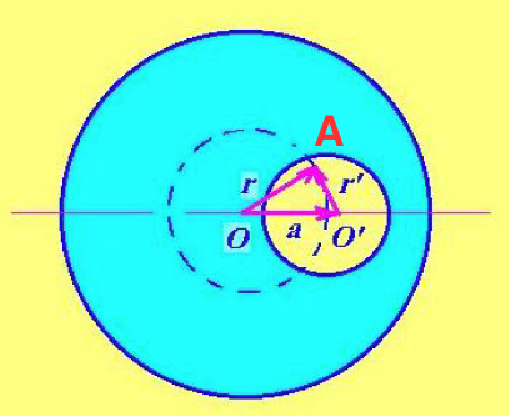
\includegraphics[width=0.35\textwidth]{image/example1.2.pdf}
\end{wrapfigure}

\noindent
\textbf{填补法},利用叠加原理\\
设想在空腔内同时填满$+\rho$和$-\rho$的电荷,则原电荷分布可视为电荷密度为$+\rho$的实心大球
和电荷密度为$-\rho$的实心小球的叠加。\\
分别做以O和O'为圆心的圆的高斯面,利用高斯定理可以求出
空腔内任意一点场强:
$$
\vec{E}_+=\frac{\rho}{3\varepsilon_0}\vec{r}\qquad\vec{E}_-=\frac{\rho}{3\varepsilon_0}\vec{r'}
$$
又因为$\vec{r}=\vec{r'}+\vec{a}$:
$$
\vec{E}=\vec{E}_+-\vec{E}_-=\frac{\rho}{3\varepsilon_0}(\vec{r}-\vec{r'})
=\frac{\rho}{3\varepsilon_0}(\vec{r}-\vec{r}+\vec{a})=\frac{\rho}{3\varepsilon_0}\vec{a}
$$
综上:
$$\vec{E}=\frac{\rho}{3\varepsilon_0}\vec{a}$$

\subsection{电势与环路定理}
\begin{theorem}
    静电场的有势性
\end{theorem}
当点电荷$q$在任意静电场中运动时,电场力的功只取决于始末位置,而与路径无关。
也就是说电场力是保守力。
这称为电场力的有势性。
\begin{wrapfigure}[4]{r}{0.4\textwidth}
    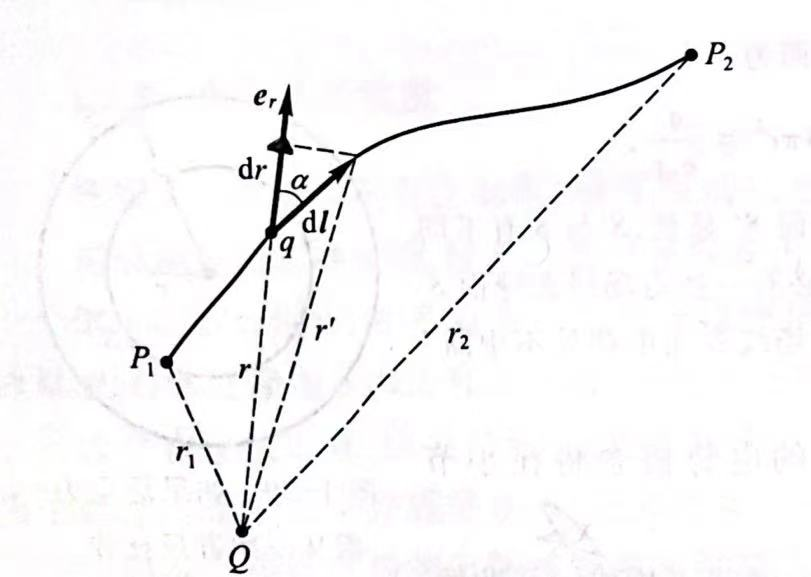
\includegraphics[width=0.4\textwidth]{image/T1_3.jpg}
\end{wrapfigure}
\begin{proof}

    \begin{align*}
        \dd W = \vec{F}\dot\dd\vec{l} =& \frac{qQ}{4\pi\varepsilon_0r^2}\vec{e_r}\dot\vec{\dd l}\\
        =& \frac{qQ}{4\pi\varepsilon_0r^2}\dd l \cos \alpha \\
        =& \frac{qQ}{4\pi\varepsilon_0r^2} \dd r
    \end{align*}

第一个等号是定义,第二个等号是库仑定律,第三,四个等号如图所示。
于是$P_1$到$P_2$的功为:
$$
W = \int_{r_1}^{r_2}\frac{qQ}{4\pi\varepsilon_0r^2}\dd r = \frac{qQ}{4\pi\varepsilon_0}(\frac{1}{r_1}-\frac{1}{r_2})
$$
可以看出只与始末位置有关,与路径无关。
\end{proof}

\begin{theorem}
    环路定理
\end{theorem}
静电场沿着任一闭合曲线的环流为零。\\
即:
\begin{equation}\label{环路定理}
\oint\vec{E}\cdot\dd\vec{l}=0
\end{equation}
\begin{proof}
    画一个闭合曲线,取两点$A$和$B$,因为静电力做功与路径无关,所以$W_{AB}$与$W_{BA}$互为相反数,
    所以$W_{all}=W_{AB}+W_{BA}=0$,所以环流为零。
\end{proof}
\begin{definition}
    电势
\end{definition}
在场内选一点$P_0$,规定$P_0$的电势为零,那么场内任一点$P$的电势$V$定义为:
\begin{equation}\label{电势}
V \equiv \frac{W}{q} = \frac 1q\int_{P}^{P_0}\vec{F}\vec{\dd l} = \int_{P}^{P_0}\vec{E}\cdot\dd\vec{l}
\end{equation}
\begin{definition}
    电势差
\end{definition}
两点之间的电势差定义为:
\begin{equation}
	\Delta V = V_A - V_B = \int_{A}^{B}\vec{E}\cdot\dd\vec{l}
\end{equation}
下面介绍两种计算电势的方法:
\begin{itemize}
    \item 用点电荷电势的计算公式
    \item 用电场的积分计算
\end{itemize}
下面一一介绍。\\
先介绍第一种方法。
\begin{theorem}
    点电荷的电势计算公式
\end{theorem}
点电荷$q$在场中某点$P$的电势为:
\begin{equation}
V =\int_{P}^{P_0}\vec{E}\cdot\dd\vec{l} = \frac{Q}{4\pi\varepsilon}\int_{r}^{\infty}\frac{\dd r}{r^2} = \frac{q}{4\pi\varepsilon_0r}
\end{equation}
写成积分形式:
\begin{equation}\label{点电荷电势}
V = \frac{1}{4\pi\varepsilon_0}\iiint\frac{\rho\dd V}{r} = \frac{1}{4\pi\varepsilon_0}\iint\frac{\sigma\dd S}{r}
\end{equation}
\begin{example}
    计算均匀带电圆盘上的电势。已知圆盘半径$R$和电荷面密度$sigma$,参考点在无限远处。
\end{example}
因为是圆盘,所以想到用极坐标。极坐标中$\dd S = R\dd\varphi\dd r$,所以:
$$
\dd V = \frac{\sigma R\dd\varphi\dd r}{4\pi\varepsilon_0\sqrt{r^2+z^2}} 
$$
注意$r$是电荷元与极坐标原点的距离,$z$是电荷元与参考点的距离。\\
积分可知:
$$
V = \iint \frac{\sigma R\dd\varphi\dd r}{4\pi\varepsilon_0\sqrt{r^2+z^2}} 
= \frac{\sigma}{4\pi\epsilon_0}\int_{0}^{2\pi}\dd\varphi\int_{0}^{R}\frac{r\dd r}{\sqrt{r^2+z^2}} 
= \frac{\sigma}{2\epsilon_0}(\sqrt{R^2+z^2}-z)
$$
下面介绍第二种。
\begin{example}
    求带电球内外电势,已知球体半径$R$和电荷密度$\sigma$。
\end{example}
由高斯定理得到电场分布:
$$
E=
\left \{
    \begin{array}{ll}
        \frac{\sigma R^3}{4\pi\varepsilon_0r^2}\vec{e_r} &(r \geqslant R)\\
        \frac{\sigma r}{3\varepsilon_0}\vec{e_r} &(r \leqslant R)\\
    \end{array}
\right .
$$
由公式(\ref{电势})可以知道:
$$
V = \int_{P}^{P_0}\vec{E}\cdot\dd\vec{l}
$$
所以:
$$
V=
\left \{
    \begin{array}{ll}
        \frac{\sigma R^3}{3\varepsilon_0}\frac 1r & (r \geqslant R)\\
        \frac{\sigma}{3\varepsilon}(R^2+R-r) & (r \leqslant R)\\
    \end{array}
\right .
$$

\begin{theorem}
  电场与电势的关系
\end{theorem}
\begin{equation}\label{电场与电势关系}
  \vec{E}=-\nabla V
\end{equation}

\newpage
\section{有导体时的静电场}
\begin{itemize}
	\item \textbf{带电导体}:总电荷不为零的导体
	\item \textbf{中性导体}:总电荷为零的导体
	\item \textbf{孤立导体}:与其他物体距离足够远的导体
\end{itemize}
\newpage
\subsection{导体静电平衡}
\begin{definition}
  导体静电平衡
\end{definition}
当导体内自由电子不做宏观运动(也就是没有电流的)的时候,我们说导体处在静电平衡状态。\\
静电平衡的必要条件是导体内部电场为零。因为如果有一点电场不为零,就会发生电荷的移动,改变电场分布,直到总电场为零。\\
这可以推出以下的性质:(当导体处于静电平衡时)
\begin{itemize}
	\item \textbf{导体内部是等势体。}\\
	这是因为导体内部电场为零,所以无论怎么移动,电场力不会做功,电势不会改变。
	\item \textbf{导体内部电荷体密度为零,电荷只分布在表面上。}\\
	在导体里选一个点,围绕这个点做一个小小的高斯面,由于电场强度是零,根据高斯定理可以知道$q_{\text{内}}=0$,所以电荷体密度为零。
	\item \textbf{在导体外部,\CJKunderdot{紧靠}导体表面的地方,电场垂直于导体表面。}

\begin{minipage}{0.5\textwidth}
	更准确的:
	\begin{equation}\label{导体表面电场}
		\vec{E}=\frac{\sigma}{\varepsilon_0}\vec{e_n}
	\end{equation}
	如图所示建立高斯面,再由高斯定理可以得到。
	$$
		S\vec{E} = \frac{\sigma S}{\varepsilon_0}
	$$
	消去$S$就可以得到了。
	\end{minipage}
	\begin{minipage}{0.5\textwidth}
		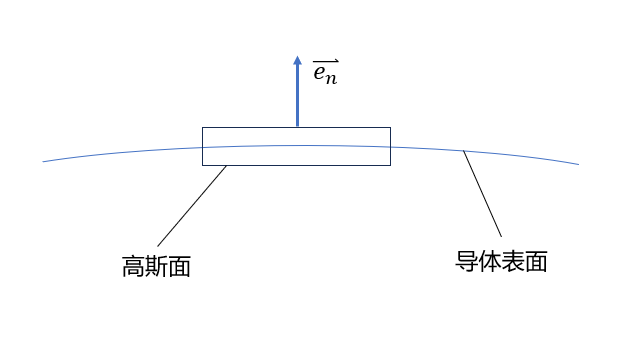
\includegraphics[width=\textwidth]{image/2.1.1.png}
	\end{minipage}
	\begin{note}
		这个式子看起来表示导体表面附近的电场强度只受导体表面的电荷影响,但实际上电场强度是由全空间的电荷影响的。
		这看似有些矛盾,导体外电荷的影响体现在哪里呢?\\
		它们可以通过改变导体表面的电荷分布来改变电场。\\
		想象一个孤立导体球,电荷面密度为$\sigma$,在它旁边放一个点电荷,那么电荷面密度就变成了$\sigma '$,这两个情况的电场强度是不同的。
	\end{note}
\end{itemize}

\subsection{带电导体所受静电力}
由公式(\ref{导体表面电场})可以知道,\textbf{紧靠}导体外一点$P'$:
$$
\vec{E}(P') = \frac{\sigma}{\varepsilon_0}\vec{e_n} = \vec{E}_{\Delta S}(P')+\vec{E}_{\text{other}}(P')
$$
其中$\vec{E}_{\Delta S}(P')$是高斯面内电荷产生的电场强度,$\vec{E}_{\text{other}}(P')$是除了高斯面内电荷的其他电荷产生的电场强度。\\
对于$P'$而言,$\Delta S$可以视为一个无限大带电平面,所以$\vec{E}_{\Delta S}(P') = \frac{\sigma}{2\varepsilon_0}\vec{e_n}$,
于是$\vec{E}_{\text{other}}(P') = \frac{\sigma}{\varepsilon_0}\vec{e_n}$(因为这俩加起来是$\frac{\sigma}{\varepsilon_0}\vec{e_n}$)\\
又因为电场在法向方向上连续,所以对于在导体上的$P$点:
$$
\vec{E}_{\text{other}}(P') = \frac{\sigma}{\varepsilon_0}\vec{e_n}
$$
根据$\vec{F} = q\vec{E} = \oint_S \sigma \vec{E} \dd S$ 就能得到导体受力了。
\begin{note}
	这实际上是导体受到外部电荷的力,所以这个结果和之前的(\ref{导体表面电场})看似有些冲突。
	(\ref{导体表面电场})是说的导体外部一点,而这里得到的是导体表面上,实际上就是导体内的一点。想明白这一点就不冲突了。
\end{note}

\subsection{平行板导体组}
这种题的步骤是根据静电平衡和导体带电量列出方程,然后再解方程就好了。
一般是带电量列一组,然后导体内找点再列一组,然后解方程。
\begin{example}
	A,B板带电分别是$q_a$,$q_b$,C不带电,求六个壁的电荷面密度。
\end{example}
\begin{wrapfigure}[6]{r}{0.3\textwidth}
		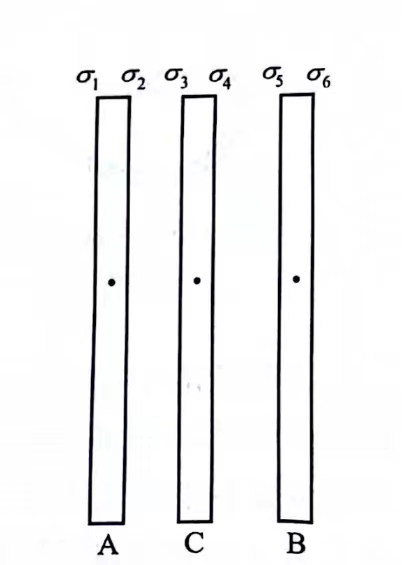
\includegraphics[width=0.3\textwidth ]{image/平行板导体组.jpg}
\end{wrapfigure}
由电荷量可以列出三个方程:
\begin{gather*}
	\sigma_1+\sigma_2 = \frac{q_a}{S}\\
	\sigma_3+\sigma_4 = 0\\
	\sigma_5+\sigma_6 = \frac{q_b}{S}
\end{gather*}
每个板内取一点,因为是导体,所以板内电场为零,也就是每个点的电场是零。又因为无限大带电平板产生的电场是$\frac{\sigma}{2\varepsilon_0}$,每个电的电场都是六个带电板叠加产生的,所以:
\begin{gather*}
	\sigma_1 - \sigma_2 - \sigma_3 - \sigma_4 - \sigma_5 - \sigma_6 = 0\\
	\sigma_1 + \sigma_2 + \sigma_3 - \sigma_4 - \sigma_5 - \sigma_6 = 0\\
	\sigma_1 + \sigma_2 + \sigma_3 + \sigma_4 + \sigma_5 + \sigma_6 = 0
\end{gather*}
解这六个方程就可以得出答案了。\textbf{提示:}把下面这三个式子加加减减就能得出$\sigma_1 = \sigma_6$,这是突破点。\\
答案是:
$$
\sigma_1 = \sigma_6 = \frac{q_a+q_b}{2S},\qquad \sigma_2 = -\sigma_3 = \sigma_4 = -\sigma_5 = \frac{q_a-q_b}{2S}
$$

\subsection{电容器及其电容}
\begin{definition}
	电容
\end{definition}
\begin{equation}
C \equiv \frac{Q}{U}
\end{equation}

几种常见的电容器的电容:
\begin{align}
	&\text{平行板电容器}\qquad
	C = \frac{\varepsilon_0S}{d}\\
	&\text{球形电容器}\qquad
	C = 4\pi\varepsilon_0\frac{R_1R_2}{R_2-R_1}\\
	&\text{圆柱形电容器}\qquad
	C = 2\pi\varepsilon_0\frac{L}{\ln\frac{R_2}{R_1}}
\end{align}
实际上都可以用平行板电容器的结果来算。\\
\begin{theorem}
	电容器连接的计算公式
\end{theorem}
\begin{itemize}
	\item \textbf{串联}:\begin{equation}\frac{1}{C}=\sum_{1}^{n}\frac{1}{C_n}\end{equation}
	\item \textbf{并联}:\begin{equation}C=\sum_{1}^{n}C_n\end{equation}
\end{itemize}
下面举一个例题看看,当时有一些没考虑到的问题。
\begin{example}
	求这个电容器组合的电容
\end{example}

\begin{wrapfigure}[6]{r}{0.5\textwidth}
	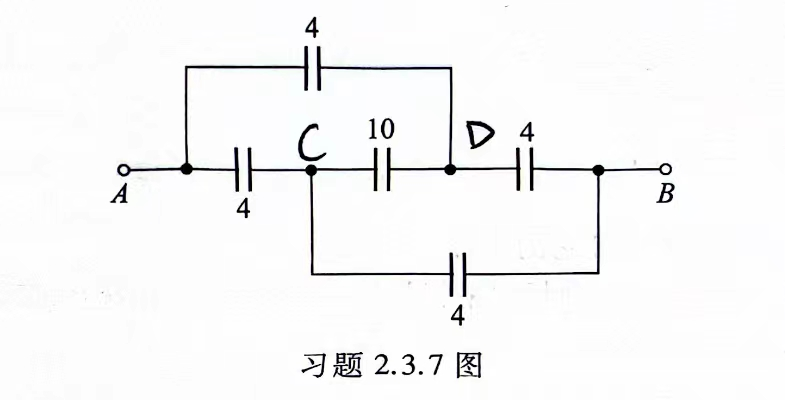
\includegraphics[width=0.5\textwidth]{image/电容器组合.jpg}
\end{wrapfigure}
分析一下就能知道C,D 两点电势相等,所以中间那个电容实际上没有,就变成了简单的串并联问题。\\
答案是$4\mu F$。
\begin{theorem}
	电容器的能量
\end{theorem}
\begin{equation}
	W = \frac{1}{2}CU^2 = \frac{Q^2}{2C} = \frac{QU}{2}
\end{equation}

\newpage
\section{静电场中的电介质}
电介质要和导体区分一下,电介质不是导体,内部没有自由电荷,没有静电平衡。\\
它的电荷是经过极化才有的,是极化电荷。
\newpage
\subsection{偶极子}
\begin{definition}
	偶极子
\end{definition}
两个相距很近而且等值异号的点电荷构成的组合叫做偶极子。
\begin{definition}
	电偶极矩(偶极矩,电矩)
\end{definition}
$\vec{l}$是从负电荷指向正电荷的矢量。
$$\vec{p} \equiv q\vec{l}$$
\begin{theorem}
	偶极子在外电场中所受的力矩
\end{theorem}
\begin{wrapfigure}[5]{r}{0.4\textwidth}
	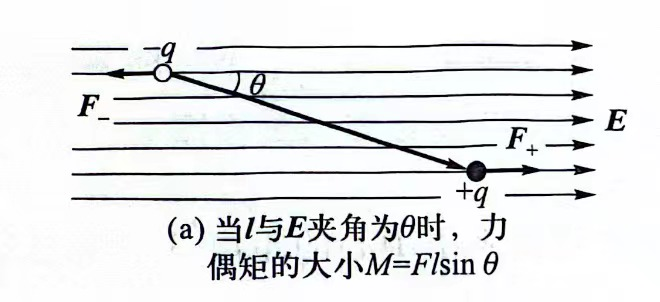
\includegraphics[width=0.4\textwidth]{image/偶极子.jpg}
\end{wrapfigure}
受到一个力偶矩:
$$\vec{M}=2\vec{F}\times\frac{\vec{l}}{2}=q\vec{l}\times\vec{E}=\vec{p}\times\vec{E}$$
这个力矩会让偶极子的电偶极矩$p$的方向趋向于$E$的方向。
\begin{theorem}
	偶极子激发的静电场
\end{theorem}
如图所示这是一个偶极子,下面求它在$P$点产生的电场。
\begin{wrapfigure}[12]{r}{0.3\textwidth}
	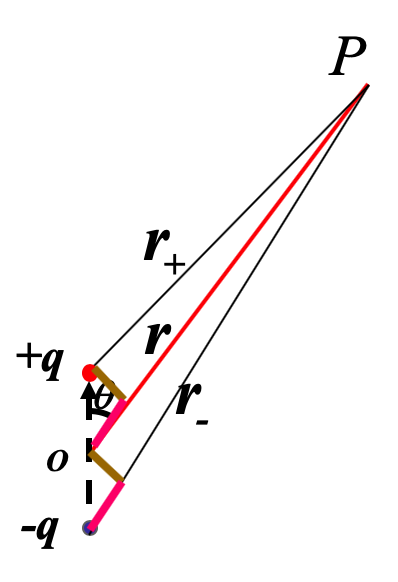
\includegraphics[scale=0.5]{image/偶极子电场.png}
\end{wrapfigure}
由点电荷电势公式(\ref{点电荷电势})可以知道:
$$V = \frac{1}{4\pi\varepsilon_0}\left(\frac{q}{r_+}-\frac{q }{r_-}\right)$$
当$r \gg l$时,可以知道$$r_+ \approx r - \frac l2 \cos\theta,\qquad r_- \approx r + \frac l2\cos\theta$$
所以:
$$
V=\frac{q}{4 \pi \varepsilon_{0}} \frac{r_{-}-r_{+}}{r_{+} r_{-}} \approx \frac{q}{4 \pi \varepsilon_{0}} \frac{l \cos \theta}{r^{2}}=\frac{\vec{p} \cdot \vec{r}}{4 \pi \varepsilon_{0} r^{3}}
$$
由电势与电场的关系(\ref{电场与电势关系})可以知道:
$$\vec{E}=-\nabla V$$
我们利用极坐标下的$\nabla$算符:(这是因为偶极子的电场是轴对称的,用球坐标很好做。)
$$
\frac{\partial}{\partial r}\vec{e_r}+
\frac 1r \frac{\partial}{\partial \theta}\vec{e_\theta}+
\frac{1}{r\sin\theta}\frac{\partial}{\partial\varphi}\vec{e_\varphi}
$$
代入可以得到:
$$
\vec{E}(\vec{r},\theta)=
\frac{p}{4 \pi \varepsilon_0 r^3}
\left(2\cos\theta\vec{e_r}+\sin\theta\vec{e_\theta}\right)
$$
\subsection{电介质的极化}
\begin{itemize}
	\item \textbf{位移极化:}正反电荷“重心”在外电场的作用下发生位移,形成极化电荷(偶极子)。
	\item \textbf{取向极化:}在外电场的作用下,有极分子的电偶极矩的方向改变(趋向外电场的方向)。
\end{itemize}
需要注意的是:极化电荷产生的电场与原来的电场是相反方向的(电偶极矩的方向和偶极子产生的电场线的方向相反)。
\begin{definition}
	极化强度
\end{definition}
\begin{equation}\label{极化强度定义}
	\vec{P} \equiv \frac{\sum \vec{p_i}}{\Delta V}
\end{equation}
\begin{theorem}
	极化强度和电场强度的关系
\end{theorem}
对于\textbf{各向同性电介质},有:
\begin{equation}
	\vec{P} = \varepsilon_0\chi\vec{E}
\end{equation}
这是实验得出来的。$\chi$是电介质的电极化率。
\subsection{极化电荷}
\begin{definition}
	极化电荷
\end{definition}
极化电荷是由于极化而产生的宏观电荷
如图所示这是一个介质的界面,可以看出来,只有被界面穿过的偶极子才对表面的极化电荷有贡献。
\begin{itemize}
	\item 在内部的没有穿过的:所有的这些偶极子的电荷代数和为零
	\item 在外部的没有穿过的:压根和这个电介质没关系(有点绝对了,但是确实和表面电荷分布没关系)
\end{itemize}

\begin{wrapfigure}[6]{r}{0.3\textwidth}
	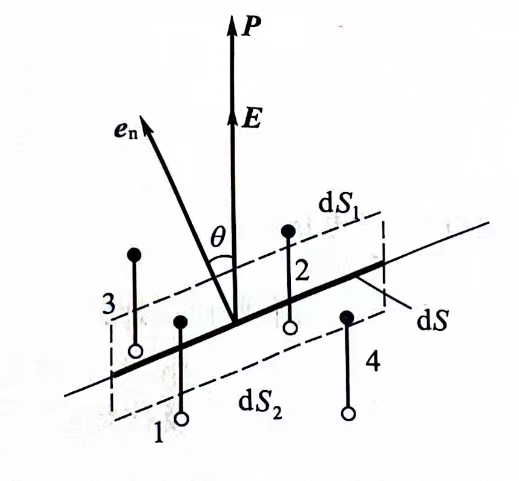
\includegraphics[width=0.3\textwidth]{image/极化电荷.jpg}
\end{wrapfigure}
下面来求一下极化电荷的量和密度。\\
虚线画出的这个体元里面,单位体积内偶极子数(偶极子数密度)为$n$,体积是$l\left |\cos \theta\right |\dd S$,所以:
$$ \dd q_p = -qnl\cos \theta \dd S $$
负号的原因是:
\begin{itemize}
	\item $\cos \theta > 0 $: 也就是如图所示的情况,对极化电荷有贡献的是负电荷,所以$q$前面加个负号,代表负电荷。
	\item $\cos \theta < 0 $: 把图中的正负电荷调转的情况,这个情况下,要算出体积,求的是$\left | \cos \theta \right |$,所以也要加个负号。
\end{itemize}
这个式子里面$nql$就是极化强度$\vec{P}$的大小,又看到这个$\cos \theta$,很自然地改写成:
$$ \dd q_p = -\vec{P}\cdot \dd \vec{S}$$
积分之后就得到\textbf{极化电荷总量}:
\begin{equation}\label{极化电荷总量}
	q_p = -\oiint_S \vec{P}\cdot \dd \vec{S}
\end{equation}
两边同时除以$\Delta V$,将$\Delta V$缩为物理无限小,就得到了\textbf{极化电荷体密度}:
\begin{equation}\label{极化电荷体密度}
	\rho_p = -\frac{\oiint_S \vec{P}\cdot \dd \vec{S}}{\Delta V} = -\nabla \cdot \vec{P}
\end{equation}
\begin{wrapfigure}[8]{r}{0.3\textwidth}
	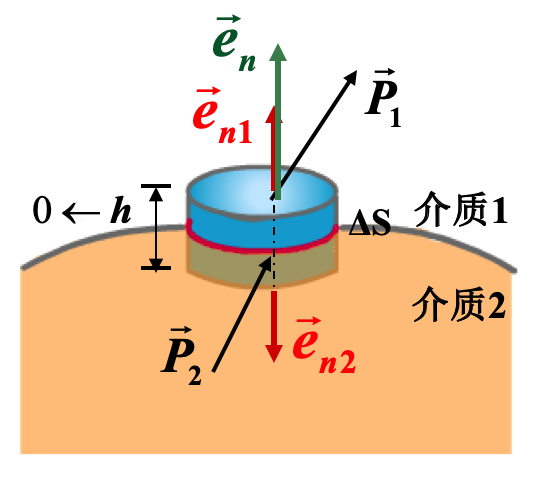
\includegraphics[width=0.3\textwidth]{image/极化电荷面密度.png}
\end{wrapfigure}
由极化电荷总量公式(\ref{极化电荷总量})可以得到:
$$
q_p = -\oiint_S \vec{P}\cdot \dd \vec{S} = -(\Delta S \vec{P_1}\cdot \vec{e_{n1}} + \Delta S \vec{P_2}\cdot \vec{e_{n2}})
$$
因为$\vec{e_{n1}} = -\vec{e_{n2}}$,命$\vec{e_n} = \vec{e_{n1}}$,所以:
$$
q_p = \Delta S \vec{P_2}\cdot \vec{e_{n}} - \Delta S \vec{P_1}\cdot \vec{e_{n}} = \Delta S (\vec{P_2}-\vec{P_1})\cdot \vec{e_{n}}
$$
又因为$q_p = \sigma_p \Delta S $,所以\textbf{极化电荷面密度}: 
\begin{equation}\label{极化电荷面密度}
	\sigma_p = (\vec{P_2}-\vec{P_1})\cdot \vec{e_{n}}
\end{equation}

\begin{example}
	均匀极化的电介质球,半径为$R$,极化强度$\vec{P}$;
	求 (1) 表面上极化电荷分布;
	(2) 极化电荷在球心处产生的电场.
\end{example}

\begin{wrapfigure}[8]{r}{0.3\textwidth}
	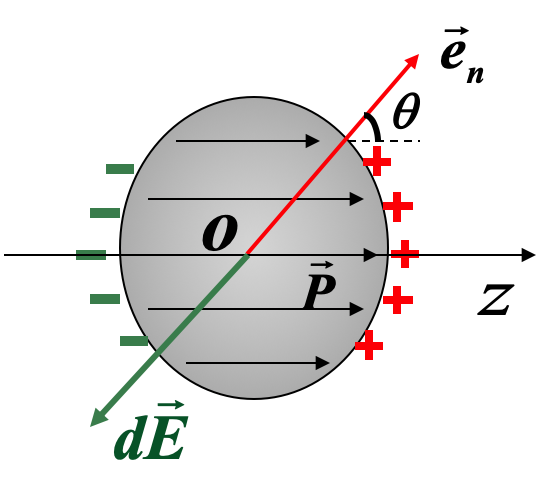
\includegraphics[width=0.3\textwidth]{image/极化电荷例题.png}
\end{wrapfigure}
(1) 由极化电荷面密度公式(\ref{极化电荷面密度})可以得到:
$$ \sigma_p = (\vec{P_2}-\vec{P_1})\cdot \vec{e_{n}} = P\cos\theta $$
(2) 由点电荷电场公式(\ref{点电荷电场})可以得到:
$$ \vec{E} = \frac{1}{4\pi\varepsilon_0}\frac{\oiint_S \sigma_p \dd S}{R^2}\vec{e_r} $$
由于是球体具有对称性,所以垂直于$z$轴方向的量相互抵消,只有$z$方向的电场强度:
\begin{align*}
	E_z &= \frac{1}{4\pi\varepsilon_0}\frac{P}{R^2}\oiint_S R^2 \cos^2 \theta \sin \theta \dd \theta \dd \varphi
		= \frac{P}{4 \pi \varepsilon_0}\int_{0}^{\pi} \cos^2 \theta \sin \theta \dd \theta \int_{0}^{2\pi} \dd \varphi\\
		&= \frac{P}{2 \varepsilon_0}\int_{0}^{\pi} \cos^2 \theta \sin \theta \dd \theta 
		= \frac{P}{2 \varepsilon_0}\int_{0}^{\pi} - \cos^2 \theta \dd \cos \theta \\
		&= \frac{P}{2 \varepsilon_0}\left.\left(-\frac{1}{3}\cos^3 \theta\right)\right|_{0}^{\pi}
		= \frac{P}{2 \varepsilon_0}\left(-\frac 13 (-1)^3 - (- \frac 13 (1)^3)\right)
		= \frac{P}{2 \varepsilon_0} \times \frac 23\\
		&= \frac{P}{3 \varepsilon_0}
\end{align*}

\subsection{有电介质时的高斯定理}
\begin{definition}
	电位移矢量
\end{definition}
\begin{equation}\label{电位移矢量}
	\vec{D} \equiv \varepsilon_0\vec{E}+\vec{P}
\end{equation}
下面说明一下电位移矢量是怎么来的。\\
当空间里有电介质的时候,要把极化电荷和自由电荷同时考虑进来,那么高斯定理就变成了:
$$
\oiint_S \vec{E} \cdot \dd \vec{S} = \frac{q_f+q_p}{\varepsilon_0}
$$
把电势$\varepsilon_0$移过去,再把$q_p = - \oiint_S \vec{P}\cdot \dd \vec{S}$代入。
$$
\oiint_S \varepsilon_0 \vec{E} \cdot \dd \vec{S} = q_f - \oiint_S \vec{P}\cdot \dd \vec{S}
$$
把带$\vec{P}$的项移到左边:
$$
\oiint_S \left( \varepsilon_0 \vec{E} + \vec{P} \right)\cdot \dd \vec{S} = q_f
$$
很自然的想要把括号里的这一串变成一个东西。\\
也就是电位移矢量$\vec{D} \equiv \varepsilon_0\vec{E}+\vec{P}$\\
所以:
\begin{theorem}
	有电介质时的高斯定理
\end{theorem}
\begin{equation}\label{介质高斯定理}
	\oiint_S \vec{D} \cdot \dd \vec{S} = q_f
\end{equation}

下面再说一下微分形式:
\begin{align*}
	&\nabla \cdot \vec{E} = \frac{\rho_f + \rho_p}{\varepsilon_0} \\
	\Rightarrow \qquad
	&\nabla \cdot \varepsilon_0 \vec{E} = \rho_f - \nabla \cdot \vec{P}\\
	\Rightarrow \qquad
	&\nabla \cdot \left(\varepsilon_0\vec{E}+\vec{P}\right) = \rho_f\\
	\Rightarrow \qquad
	&\nabla \cdot \vec{D} = \rho_f
\end{align*}
把$\vec{P} = \varepsilon_0\chi\vec{E}$代入$\vec{D} \equiv \varepsilon_0\vec{E}+\vec{P}$,就可以得到:
$$
\vec{D} = \varepsilon_0 \left(1 + \chi \right) \vec{E}
$$
\begin{definition}
	介电常量和相对介电常量
\end{definition}
介电常量:
\begin{equation}\label{介电常量}
	\varepsilon \equiv \varepsilon_0\left(1 + \chi \right) 
\end{equation}
相对介电常量:
\begin{equation}
	 \varepsilon_r \equiv \frac{\varepsilon}{\varepsilon_0} = 1 + \chi
\end{equation}
把(\ref{介电常量})代入$\vec{D} = \varepsilon_0 \left(1 + \chi \right) \vec{E}$:
\begin{equation}
	\vec{D} = \varepsilon \vec{E} = \varepsilon_0 \varepsilon_r \vec{E}
\end{equation}
\begin{note}
	解决电介质问题的步骤:
\end{note}
\begin{itemize}
	\item 通过高斯定理求出$\vec{D}$
	\item 通过$\vec{D} = \varepsilon \vec{E} = \varepsilon_0 \varepsilon_r \vec{E}$求出$\vec{E}$
	\item 通过$\varepsilon_0 \chi \vec{E} = \varepsilon_0(\varepsilon_r - 1) \vec{E} = \vec{P}$求出$\vec{P}$
	\item 通过$\rho = -\nabla \cdot \vec{P}$或者$\sigma = (\vec{P_2}-\vec{P_1})\cdot \vec{e_{n}}$求出极化电荷分布
	\item 通过$\vec{E} = \frac{1}{4\pi\varepsilon_0}\frac{q}{r^2}\vec{e_r}$求出极化电场,也能通过$\vec{E} = \vec{E_f} + \vec{E_p}$求出自由电荷激发的电场。
\end{itemize}
\begin{example}
	(真空中)厚度为$d$、相对介电常数为$\varepsilon_r$的无限大均匀电介质平板内以体密度$\rho_f$均匀分布自由电荷,
	求电介质板内的$\vec{E},\vec{D},\vec{P}$。
\end{example}

\begin{wrapfigure}[10]{r}{0.3\textwidth}
	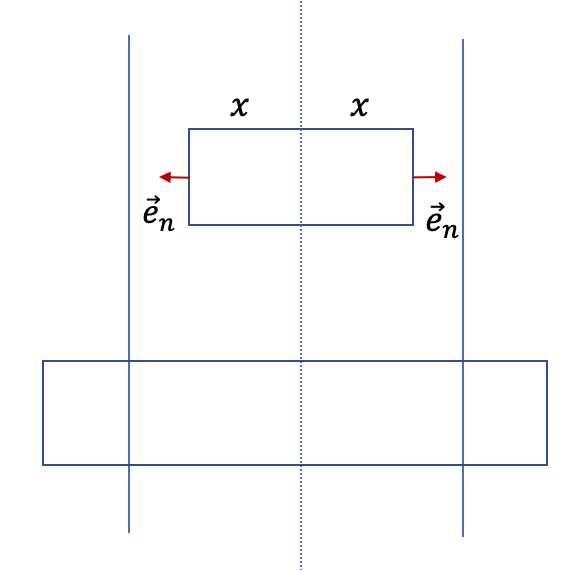
\includegraphics[width=0.3\textwidth]{image/电介质高斯定理例题.png}
\end{wrapfigure}
如图所示在平板内部建立高斯面,由高斯定理可以得到:
$$
2 D S = 2 x S \rho_f
$$
即
$$
\vec{D} = \rho_f x \vec{e_n}
$$
$\vec{e_n}$的方向是背离介质平板的方向。\\
因为$\vec{D} = \varepsilon_0 \varepsilon_r \vec{E}$,所以:
$$
\vec{E} = \frac{x \rho_f}{\varepsilon_0 \varepsilon_r}\vec{e_n}
$$
又因为$\vec{P} = \varepsilon_0(\varepsilon_r - 1) \vec{E}$所以:
$$\vec{P} = \frac{\varepsilon_r - 1}{\varepsilon_r} \rho_f x \vec{e_n}$$
\end{document}

